\chapter{Programación PLC}
\label{ch:progPLC}
Como se prensento en el capitulo \ref{ch:intro} de este informe el material a utilizar
para poder alcanzar los objetivos. En el presente capítulo se describe el algoritmo 
de programación del programa que se grabo en el \gls{plc}
\section{Algoritmo}
\label{sec:Algoritmo}



\usetikzlibrary{trees}
\tikzstyle{every node}=[draw=black,thick,anchor=west,inner sep=2pt,minimum size=1pt]
\tikzstyle{selected}=[draw=cyan,fill=cyan!30]
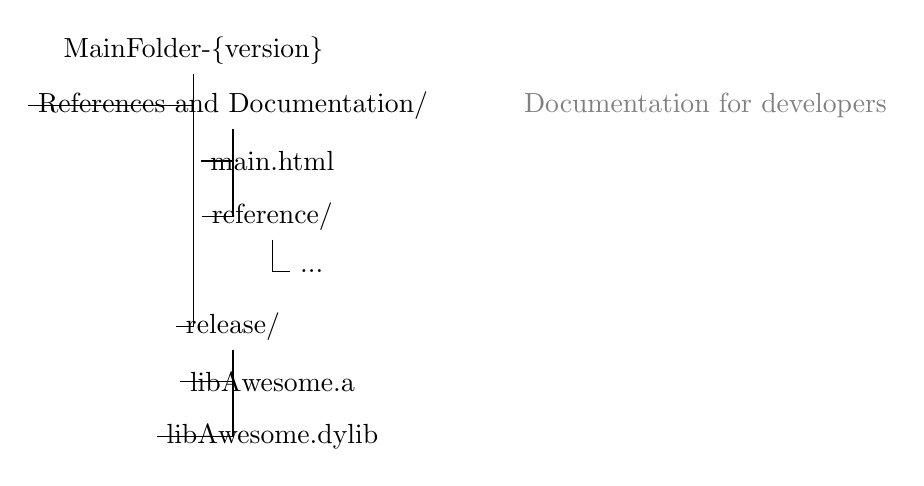
\begin{tikzpicture}[
  grow via three points={one child at (0.5,-0.7) and
  two children at (0.5,-0.7) and (0.5,-1.4)},   
  edge from parent path={(\tikzparentnode.south) |- (\tikzchildnode.west)}]
  \node {MainFolder-\{version\}}
    child { node [label={[xshift=6.0cm, yshift=-0.58cm, color=gray] Documentation for developers}] {References and Documentation/}
        child { node [draw=none] {main.html} }
        child { node {reference/}
            child { node [draw=none] {...}}
        }
        child [missing] {}
    }
    child [missing] {}
    child [missing] {}
    child [missing] {}
    child { node {release/}
        child { node [draw=none] {libAwesome.a} }
        child { node [draw=none] {libAwesome.dylib} }
    };
\end{tikzpicture}
\tikzstyle{every node}=[] % resets borders of tables
\tikzstyle{selected}=[] % resets selected






\section{Programación}
\label{sec:Programacion}
Grabado y puesta en el plc

\section{Depuración (Debug)}
\label{sec:Debug}
Forzar entradas
